\chapter{Multiplicity properties of the Galactic WNE population}\label{ch:wne}

\textit{The work presented in this chapter is based on:}

\textbf{A spectroscopic multiplicity survey of Galactic Wolf-Rayet stars: II. The northern WNE sequence}

\textbf{K. Dsilva}, T. Shenar, H. Sana and P. Marchant

Accepted for publication in {\sc Astronomy and Astrophysics},

Originally published as: \newline
arXiv:2204.12518 [astro-ph]

\textbf{Author contributions:} K. Dsilva performed the data reduction and computed the radial velocities in this chapter with the guidance of H. Sana and T. Shenar. The Monte-Carlo simulations were run by H. Sana. The Bayesian framework was developed by P. Marchant and H. Sana. All the authors assisted with the evolutionary interpretations of the presented results and contributed significantly to the text, which was written by K. Dsilva.
\newpage
\begin{abs}
\vspace{3mm}
\textbf{Original abstract:}
\newline \newline
Most massive stars reside in multiple systems that will interact over the course of their lifetime. This has important consequences on their future evolution and their end-of-life products. Classical Wolf-Rayet (WR) stars represent the final end stages of stellar evolution at the upper-mass end. While their observed multiplicity fraction is reported to be ${\sim}0.4$ in the Galaxy, their intrinsic multiplicity properties and the distributions of their orbital parameters remain insufficiently constrained to provide a reliable anchor to compare to evolutionary predictions.
  \newline \newline% aims heading (mandatory)
As part of a homogeneous, magnitude-limited ($V\leq12$) spectroscopic survey of northern Galactic WR stars, this paper aims to establish the observed and intrinsic multiplicity properties of the early-type nitrogen-rich WR population (WNE), including estimates of the multiplicity fraction and the shape of their orbital period distribution. Additionally, we compare these with the properties of the carbon-rich WR population (WC) stars obtained in the first paper of this series.
 \newline \newline% methods heading (mandatory)
We obtained high-resolution spectroscopic time series of the complete magnitude-limited sample of 16 WNE stars observable with the 1.2\,m Mercator telescope at La Palma, typically providing a time base of about two to eight years. We measured relative radial velocities (RVs) using cross-correlation and used RV variations to flag binary candidates. Using an updated Monte Carlo method with a Bayesian framework, we calculated the three-dimensional likelihood for the intrinsic binary fraction (\fintWNE{}), the maximum period (\logPmax{}), and the power-law index for the period distribution ($\pi$) for the WNE population with \Pmin{} fixed at 1\,d. We also used this updated method to re-derive multiplicity parameters for the Galactic WC population.

  % results heading (mandatory)
Adopting a peak-to-peak RV variability threshold of 50\,\kms{} as a criterion, we classify 7 of the 16 targets as binaries. This results in an observed multiplicity fraction (\fobsWNE{}) of 0.44\,$\pm$\,0.12. Assuming flat priors, we derive the best-fit multiplicity properties \fintWNE{}\,$= 0.56\substack{+0.20 \\ -0.15}$, \logPmax{}\,$= 4.60\substack{+0.40 \\ -0.77}$ , and $\pi$\,$= -0.30\substack{+0.55 \\ -0.53}$ for the parent WNE population. We explored different mass-ratio distributions and note that they did not change our results significantly. For the Galactic WC population from Chapter\,\ref{ch:wc}, we re-derive \fintWC{}\,$= 0.96\substack{+0.04 \\ -0.22}$, \logPmin{}\,$= 0.75\substack{+0.26 \\ -0.60}$, \logPmax{}\,$= 4.00\substack{+0.42 \\ -0.34}$ , and $\pi$\,$= 1.90\substack{+1.26 \\ -1.25}$.
  % conclusions heading (optional), leave it empty if necessary
The derived multiplicity parameters for the WNE population are quite similar to those derived for main-sequence O binaries but differ from those of the WC population. The significant shift in the WC period distribution towards longer periods is too large to be explained via expansion of the orbit due to stellar winds, and we discuss possible implications of our results. Analysis of the WNL population and further investigation of various evolutionary scenarios is required to connect the different evolutionary phases of stars at the upper-mass end.
\end{abs}

\section{Introduction}

According to the Conti scenario, single O stars will strip themselves of their envelope through their stellar winds and evolve spectroscopically into WN, WC and if massive enough, WO stars before ending their lives via core-collapse. However, the effect of multiplicity on this scenario and in general, massive star evolution, is not well constrained. While the intrinsic multiplicity properties of the main-sequence O population are well known, those for the WR population remain largely unconstrained. To remedy this, we undertook a spectroscopic monitoring campaign of 39 Galactic northern WR stars. In this chapter, we improve the methods explained in Chapter \ref{ch:introduction} and analyse the 16 WNE stars in our sample. We also revisit the 12 WC stars from Chapter \ref{ch:introduction}, and discuss evolutionary consequences based on our results.

\section{Sample and data reduction} \label{sect:sample_WNE}
\subsection{Sample}

We define the sub-class WNE as WN stars with spectral types equal to or earlier than WN5. In cases where objects are classified as `WN5-WN6' in the GCWR, we consider them as WN5 for simplicity. As in Chapter \ref{ch:wc}, we used $V\,\leq\,12$ or $\varv\,\leq\,13$ and declination $\delta \ge$ $-30\degree$ as our selection criteria. This resulted in a magnitude-limited sample of 16 WNE stars whose known properties are summarised in Table \ref{tab:WN_data}. Their spectral-type distribution is shown in Fig. \ref{fig:target_dist_WNE}. We obtained at least six epochs of each of the target stars. When available, we used archival HERMES observations in the RV analysis, which reach a typical time base of two to eight years. The number of spectra and the sampling time of the observations are shown in Table \ref{tab:wr_epochs}. \b{The division of the sample into WNE and WNL (WN6 and later) parts fits in the Conti scenario, which predicts evolution from WNE to WNL spectral types. However, analysis based on the morphology of the spectra, i.e. strong- and broad-lined versus weak- and narrow-lined WN stars is an alternative partitioning of the WN sample which we do not explore.}

\begin{figure}[!h]
    \centering
    %referee version
    % \includegraphics[width=0.7\textwidth]{Figures/target_dist.pdf}
    %two column version
    \includegraphics[width=0.6\textwidth]{chapters/WNE/image/target_dist.pdf}
    \caption{Distribution of spectral types within the present WNE sample.}
    \label{fig:target_dist_WNE}
\end{figure}


\subsection{Data reduction and normalisation}
The data reduction procedures for our spectra are comprehensively described in Chapters \ref{ch:introduction} and \ref{ch:wc}. After this step, what remains is the effect of interstellar reddening superimposed on the continuum from the wind. The normalisation of the spectra was performed in a similar manner to Chapter \ref{ch:wc}.

We used a model of a normalised spectrum of a WNE star from the Potsdam Wolf-Rayet code \citep[PoWR:][]{grafener_line-blanketed_2002,hamann_temperature_2003,2004HamannGrafenerWN,2015TodtWNmodels} to identify pseudo-continuum regions, in the blue around 5300\,\r{A} and in the red around 8100\,\r{A}. We then anchored the stellar continuum model for the same WNE star to the red point and applied a reddening to fit the slope. We explored various reddening laws and R$_V$ values and realised that they did not significantly impact the homogeneity of the normalisation process. Therefore, as in Chapter \ref{ch:introduction}, we used the reddening law from \citet{2004Fitzpatrick} and R$_V$ of 3.1, the average for the galaxy.

\begin{table}
\centering
\caption{List of WNE stars in our RV monitoring campaign, providing the number of spectra, time coverage, and average signal-to-noise (S/N) per resolution element at 4400\,\r{A} ($\Delta\lambda\,\simeq\,$0.05 \r{A}).}
\begin{tabular}{cccc}
\hline \hline
WR\#&Spectra&Time coverage (d)&Average S/N \\ \hline
1&27&1264&40 \\
2&18&1085&45 \\
3&8&120&70 \\
6&28&1025&120 \\
7&7&642&45 \\
10&6&678&60 \\
110&11&1142&50 \\
127&11&2646&80 \\
128&10&1120&80 \\
133&21&2890&200 \\
138&40&2898&100 \\
139&34&2954&150 \\
141&14&2140&50 \\
151&6&924&20 \\
152&7&921&40 \\
157&12&2168&70 \\ \hline

\end{tabular}
\label{tab:wr_epochs}
\end{table}

\section{Measuring radial velocities}\label{sect:RVdet_WNE}
Deriving RVs of WR stars is not a trivial process given their strong, broad emission lines that form in their outflowing winds. Of the methods that are used extensively in the community, we used cross-correlation as our tool of choice, with a statistical framework that allows us to derive meaningful uncertainties on our RV measurements \citep[][see Chapter \ref{ch:wc} for more details]{2003Zucker}. As mentioned in Chapter \ref{ch:wc}, we focus on the RVs of the WR star even in SB2 systems to maintain homogeneity in the analysis and to focus on binary detection instead of orbital analysis. We briefly describe the formulation and assumptions of the CCF.

\subsection{Cross-correlation and mask selection}
The CCF is the convolution of a chosen template to the data to measure the velocity shift. It is represented by a log-likelihood function, where the maximum is the RV of the spectrum. The uncertainty on the RV measurement can then be derived from maximum log-likelihood theory. An implicit assumption of the method is that the template accurately reproduces the data. Because WR models often do not to accurately represent the shape of both strong and weak lines simultaneously, we chose the highest signal-to-noise (S/N) epoch as the template. The measured RVs were then used to construct a weighted co-added spectrum of a higher S/N. This process was iterated until the derived RVs no longer changed significantly within the measurement errors, at which point the final template and measurements were converged. The S/N of the template contributes significantly to the measured uncertainty, and this was minimised by creating a high S/N co-added spectrum. A caveat is that the RVs derived in this fashion are relative RVs. While this is sufficient for binary detection, an absolute shift must be applied when comparing to RVs from the literature.

When compared with the WC stars analysed in Chapter \ref{ch:wc}, the WNE stars in our sample exhibit stronger line-profile variability in their spectra \b{on average, although WR 6 is an example of an outlier}. Therefore, the assumption that the template accurately represents the data often breaks down for variable stars. This directly results in larger uncertainties on the derived RVs. In order to ensure that the templates can represent the data as accurately as possible, for each star we selected encompassing spectral lines that are least affected by line-profile variability. Depending on how variable the stars are, we used lines of \niv, \nv, \heii,{} and when possible, Balmer lines. In cases of strong line-profile variability, we tend to only use \nv{} lines and occasionally \niv{} lines because they are thought to form in the hotter, inner regions of the stellar wind \citep[see, e.g.][]{1987Hillier_WN,1988Hillier}. We used a combination of all the different lines of various strengths and ions used to measure RVs and call this mask `full spec' (e.g. a combination of \nv{}, \niv,{} and \heii{} lines).

\begin{figure}
    \centering
    %referee version
    % \includegraphics[width=0.9\textwidth]{Figures/WR138_nogrid.pdf}
    \includegraphics[width=\textwidth]{chapters/WNE/image/WR138_nogrid.pdf}
    % 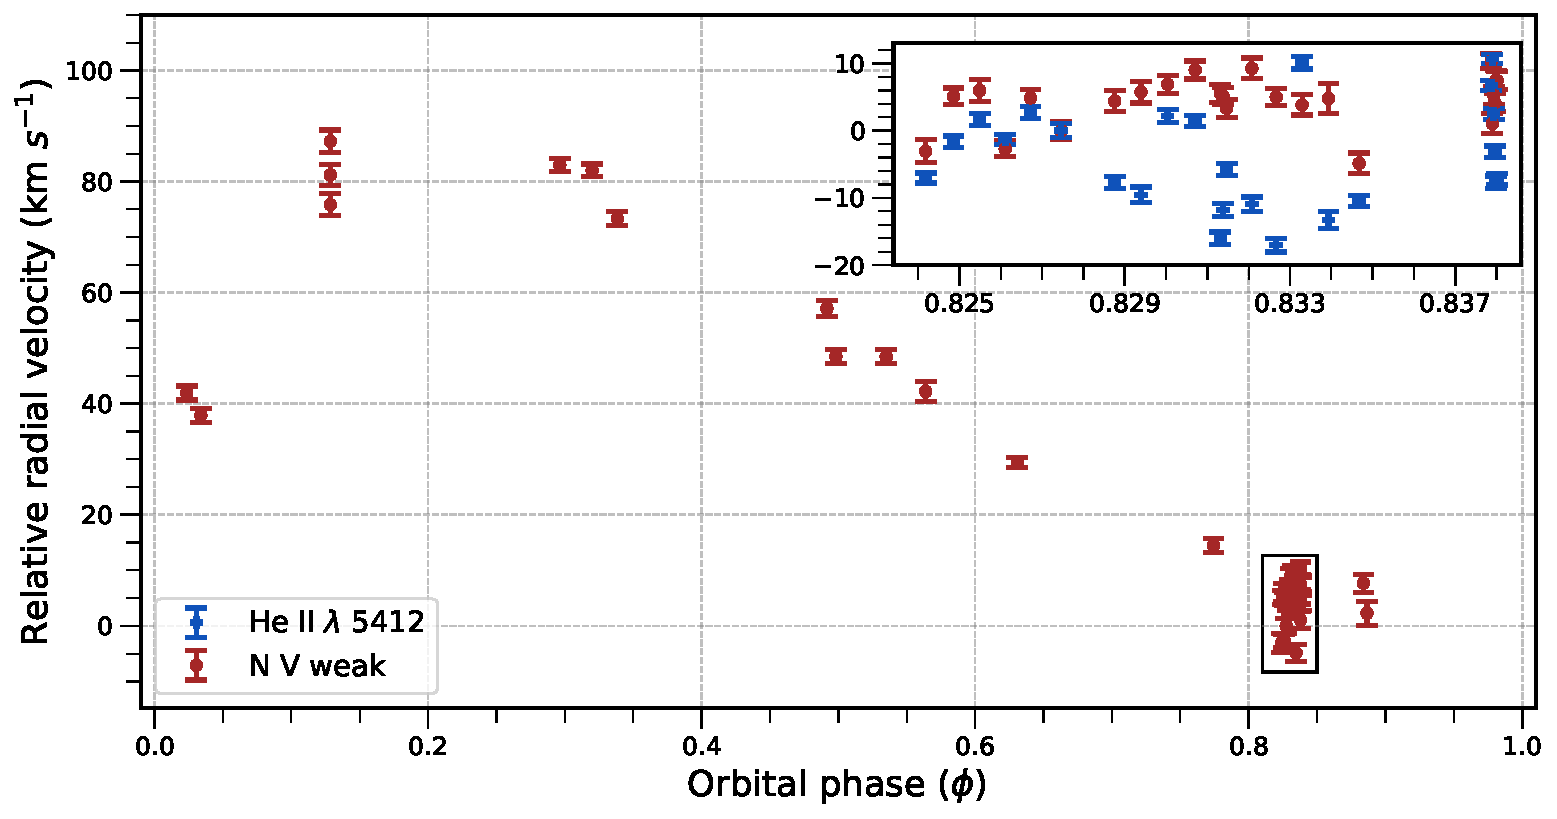
\includegraphics[width=0.49\textwidth]{Figures/WR138.pdf}
    \caption{Phased RV plot for WR 138 with HERMES data. The inset shows the high-cadence measurements (black box) with the \nv{} weak lines and the He\,{\sc ii}\,$\lambda 5412$ line. The ephemeris used for the periastron passage was JD 2445284 \citep{1990Annuk}, with the period of 1521.2\,$\pm$\,35\,d from \citet{2013Palate}.}
    \label{fig:WR138_phased}
\end{figure}

\begin{figure}[t]
    \centering
    % \includegraphics[width=0.9\textwidth]{Figures/RV_SC_ions_nogrid.pdf}
    \includegraphics[width=\textwidth]{chapters/WNE/image/RV_SC_ions_nogrid.pdf}
    % 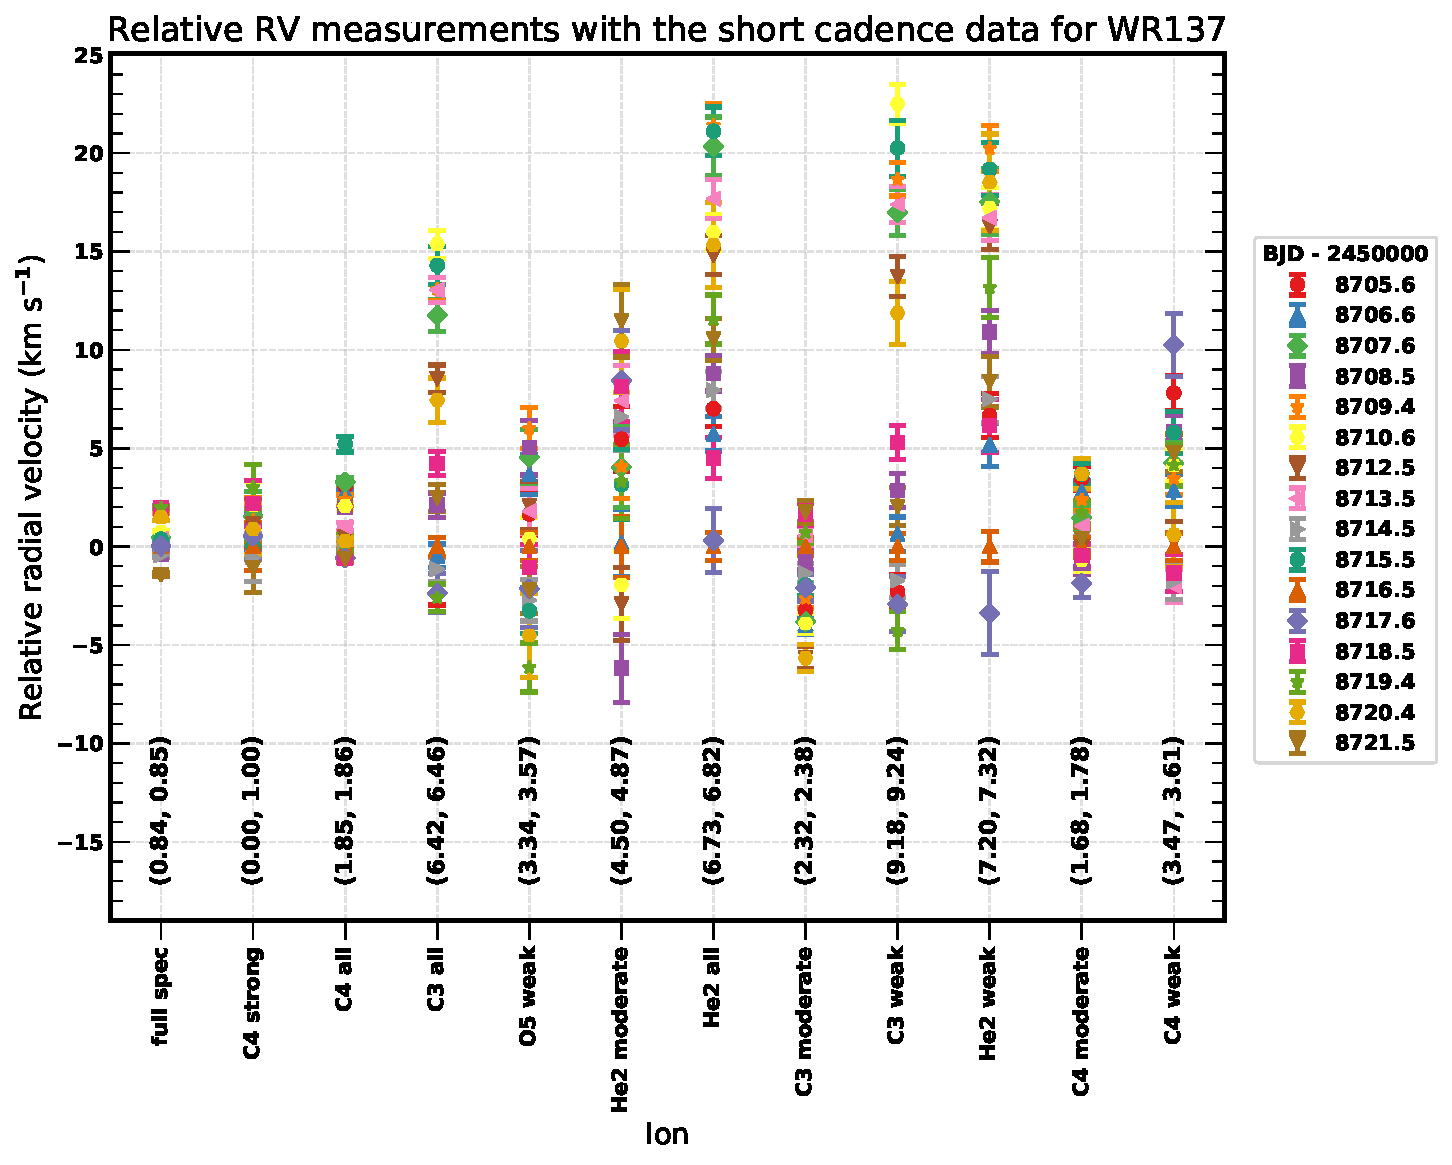
\includegraphics[width=0.49\textwidth]{Figures/RV_SC_ions.pdf}
    \caption{High-cadence relative RV measurements for WR 138 using different masks. At the bottom of the plot are the values of ($\sigma_w$, $\sigma_{\textrm{RV}}$) (\kms{}) for each mask. As mentioned in the text, `full spec' is a combination of all the masks to its left and not the entire spectrum. The \niv{} line at 5205\,\r{A} is very weak, which explains its high scatter.}
    \label{fig:sc_ions}
\end{figure}
%Looking at the values of $\sigma_w$, `full spec' and `N5 weak' masks are least affected by wind variability.
\subsection{Studying the long-period binary system WR 138 to quantify wind variability} \label{sect:windVariability}

In Chapter \ref{ch:wc}, we analysed high-cadence data of the long-period binary system WR 137 in order to understand the effect of wind variability and other systematic effects on the RV measurements. As a nitrogen-rich analogue, we studied the long-period binary WR 138 (WN5o\,+\,O9V) with a period of 4.16\,yr and a low eccentricity of 0.3 \citep{2013Palate,1990Annuk,2016Richardson}. \citet{2013Palate} also studied the system in X-rays, concluding that its emission is normal for a colliding-wind WR\,+\,OB binary system, although the sampling of their data did not allow them to check for the existence of phase-locked variability of the X-ray emission.

With this in mind, we collected high-cadence HERMES data in August of 2019 (with the periastron passage in June 2020). In total, we obtained 18 spectra over 16 consecutive nights and 6 spectra over one night a few days later (Table \ref{tab:WR138}). The phased RV plot of WR 138 is shown in Fig. \ref{fig:WR138_phased} with an emphasis on the high-cadence data over different masks. Because the high-cadence data were collected at the orbital phase of 0.8, the effect of wind-wind collision \citep[e.g.][]{2002Luehrs} on the measured RVs could be significant. Using the systemic and stellar parameters \citep{1990Annuk,2016Richardson}, we computed the cooling parameter $\chi$ \citep{1992Stevens} and found the shocked region to be adiabatic. As the cooling timescale is longer than the escape timescale, the contribution to recombination lines in the optical is minimal. Therefore, the contribution of wind-wind collision to the RV measurements should not change significantly over the timescale of the high-cadence observations. Even if wind-wind collision were to contribute significantly to the RV measurements, the derived scatter in the high-cadence study would be an upper limit on the intrinsic wind variability of the WR star.

% Since the star was significantly away from periastron at the time, we neglect the effect of wind-wind collision \citep[e.g.][]{2002Luehrs} and study the effect of the intrinsic wind variability on the RV measurements.

For the high-cadence data, the contributions to the uncertainties in the measured RVs are statistical (i.e. from the method, $\sigma_p$) and physical (i.e. from the wind physics, $\sigma_w$). The weighted standard deviation of the high-cadence measurements are indicative of the true error, which we denote by $\sigma_{\textrm{RV}}$. Assuming $\sigma_p$ and $\sigma_w$ are uncorrelated, they can simply be added quadratically as described in Eq. \ref{eq:sig_RV}.

For each mask, $\sigma_p$ is calculated from the co-variance matrix of the CCF (Eq. \ref{eq:errorCCF}). Using Eq. \ref{eq:sig_RV} along with the calculated values of $\sigma_p$ and $\sigma_{\textrm{RV}}$, we obtain an estimate for $\sigma_w$. The high-cadence data therefore allow us to isolate and quantify the effect of wind variability on the RV measurements. The lines that are least affected by wind variability are \nv{} weak lines (Appendix. \ref{apdx:comments_WNE}, $\sigma_w{\sim}\,5$\,\kms{}). Lines of \heii{} and \niv{} lines are found to be more variable ($\sigma_w{\sim}\,10$\,\kms{}). As their formation regions can be spatially different, these measurements can be helpful probes of turbulence and other physical processes. The difference in dispersion for lines of \niv{} arise from the different line strengths and since the S/N in the blue is much lower than in the red. The mask `full spec' is a combination of the \niv{}, \heii,{} and \nv{} lines. The mask `N4 7109' covers the triplet \NIVred{}. Ultimately, we chose to measure RVs for WR 138 using weak \nv{} lines, namely a combination of \NVblue,{} and \NVred{}.

Although we observed that weak \nv{} lines showed the least intrinsic variability for WR 138, this  cannot necessarily be generalised for all WNE stars. However, for all the objects in our sample, we realised that the \nv{} lines indeed had the least RV dispersion, and we therefore used them to measure RVs. For stars with strong line-profile variability (WR 2, WR 6, WR 7, and WR 110), we used the combination of all masks (`full spec') to measure RVs (Appendix.\,\ref{apdx:comments_WNE}). The full journal of RV measurements for each object with their respective masks is given in Appendix.\,\ref{s:tables_RV}.

\begin{figure}[t]
    \centering
    %referee version
    % \includegraphics[width=0.9\textwidth]{Figures/BINFRAC_WN_NOGRID.pdf}
    \includegraphics[width=\textwidth]{chapters/WNE/image/BINFRAC_WN_NOGRID.pdf}
    % \includegraphics[width=0.49\textwidth]{Figures/BINFRAC_WN.pdf}
    \caption{Non-parametric threshold plot showing the inverse cumulative distribution of peak-to-peak RV variability in our sample, which is equivalent to the observed binary fraction (\fobsWNE{}) as a function of the adopted peak-to-peak RV variability threshold $C$. Names in bold are known binaries with established spectroscopic periods for the WR components.}
    \label{fig:binfrac}
\end{figure}
\begin{sidewaystable}
\small
\setlength{\tabcolsep}{0pt}
\centering
\caption{Overview of the known multiplicity properties of our sample of WNE stars together with the results of our RV measurements. \DelRV{} and $\sigma_{\textrm{RV}}$ are calculated in this work and are used to identify tentative spectroscopic binaries. The spectral types are taken from the GCWR unless indicated otherwise. The binary status of this work is reported based on the spectroscopic observations.}

\begin{threeparttable}
% \begin{tabular*}{\textwidth}{ l @{\extracolsep{\fill}} *{8}{d{0.1}} }
\centering
\begin{tabular*}{\textwidth}{l @{\extracolsep{\fill}}*{9}{c}}
% \begin{tabular*}{ccccccccc}
\toprule
\toprule

WR\# & Spectral Type & \multicolumn{2}{c}{Binary Status} & Period & e & $\Delta$ RV  & $\sigma_{\textrm{RV}}$ & \DelRV{} $>$ C\\
 & (GCWR) & (GCWR) & This work & (d) & &(\kms{}) &(\kms{}) &  \\ \midrule
1 & WN4 & SB1? & - & - & - & 37.5 & 8.6 & no\\
2 & WN2 & VB & VB\tnote{(l)} & - & - & 36.9 & 8.3 & no\\
3 & WN3ha & SB2 & - & -\tnote{(a)} & - & 5.0 & 1.8 & no\\
%3 & WN3ha & SB2 & no & 46.85$\pm$0.02\tnote{(a)} & 0 (fixed)\tnote{(a)} & 5.0 & 1.8\\
6 & WN4b & SB1 & SB1 & 3.8\tnote{(b)} & 0.1\tnote{(b)} & 170.0 & 40.3 & yes\\
7 & WN4b & - & - & - & - & 33.3 & 10.8 & no\\
10 & WN5h & VB & VB\tnote{(l)} & - & - & 9.9 & 3.6 & no\\
110 & WN5b & - & - & - & - & 31.8 & 11.3 & no\\
127 & WN3b\,+\,O9.5V & SB2 & SB2 & 9.5550\,$\pm$\,0.0002\tnote{(c)} & 0.04\,$\pm$\,0.02\tnote{(c)} & 332.0 & 108.9 & yes\\
128 & WN4(h) & SB2?, VB & VB\tnote{(l)} & - & - & 9.7 & 2.8 & no\\
133 & WN5o\,+\,O9I & SB2, VB & SB2, VB\tnote{(l)} & 112.780\,$\pm$\,0.036\tnote{(d)} & 0.3558\,$\pm$\,0.0050\tnote{(d)} & 111.6 & 25.8 & yes\\
138 & WN5o\,+\,O9V\tnote{(e)} & SB2, VB & SB2, VB\tnote{(l)} & 1521.2\,$\pm$\,35\tnote{(f)} & 0.3\tnote{(g)} & 92.1 & 29.4 & yes\\
139 & WN5o\,+\,O6III-V & SB2 & SB2 & 4.212435\tnote{(h)} & 0.036\,$\pm$\,0.009\tnote{(h)} & 618.3 & 168.9 & yes\\
141 & WN5o\,+\,O5V-III & SB2 & SB2 & 21.6895\,$\pm$\,0.0003\tnote{(i)} & 0.018\,$\pm$\,0.035\tnote{(i)} & 209.8 & 66.5 & yes\\
151 & WN4o\,+\,O5V & SB2 & SB2 & 2.12691\,d\tnote{(j)} & 0 (fixed)\tnote{(j)} & 650.0 & 220.7 & yes\\
152 & WN3(h) & - & - & - & - & 8.3 & 2.6 & no\\
157 & WN5o\,+\,(B0.7II\,+\,B1III)\tnote{(k)} & VB & SB3, VB\tnote{(l)} & - & - & 11.8 & 3.6 & no\\
\bottomrule
\end{tabular*}
\begin{tablenotes}
   \item[(a)] \citet{1986Moffat+abs} reported a period of 46.8\,d, but it is not supported by our analysis (App. \ref{apdx:comments_WNE}),
    \item[(b)] \citet{2020Koenigsberger},
    \item[(c)] \citet{2011delachevrotiere},\\
    \item[(d)] \citet{2021Richardson},
    \item[(e)] \citet{2016Richardson},
    \item[(f)] \citet{2013Palate},
    \item[(g)] \citet{1990Annuk},
    \tnote{(h)} \citet{1994Marchenko}\,[fixed P; 4.212435\,d],\\
    \tnote{(i)} \citet{1998Marchenko1998WR141},
    \tnote{(j)} \citet{2009HuttonWR151},
    \tnote{(k)} \citet{2021MaizAppelaniz},
    \tnote{(l)} VB status carried over from the GCWR.
\end{tablenotes}
\end{threeparttable}
\label{tab:WN_data}
\end{sidewaystable}


\section{Observed binary fraction}\label{sect:results_WNE}

For each star in our sample, we measured the RVs and obtained their peak-to-peak variability amplitude (\DelRV{}). We then selected a threshold to determine the boundary beyond which the RV amplitude would be dominated by orbital motion in a binary system. We plot the binary fraction as a function of this threshold in a non-parametric threshold plot (Fig.\,\ref{fig:binfrac}). By moving the threshold from higher to lower RV values (right to left in Fig.\,\ref{fig:binfrac}), we classify more stars as RV variable, hence putative spectroscopic binaries. A summary of the characteristics of the WNE stars in our sample can be found in Table \ref{tab:WN_data}. As we cannot verify the status of objects classified as visual binaries (VB) in the GWCR, we simply carry over their status in our classification.

The next step was to choose an adequate value for the threshold $C$ such that stars with \DelRV{}$\ge$\,$C$ were classified as binaries. It is important that the chosen threshold avoids false positives, in particular, those that are erroneously classified as binaries due to strong intrinsic variability. The high-cadence study of WR 138 is a useful guideline to ensure this. The peak-to-peak RV amplitude measured due to wind variability was observed to be 15\,\kms{} for the \nv{} lines (Fig. \ref{fig:sc_ions}). We therefore chose a conservative threshold larger than three times this value, that is, 50\,\kms{}. This results in 7 of the 16 observed binaries in the sample, \fobsWNE{} $= 0.44$ with a binomial error of $\pm$\,0.12. Interestingly, all the known spectroscopic binaries in our sample with an established orbital solution are properly identified with the adopted threshold. For objects with \DelRV{}\,$<$\,50\,\kms{} and a large enough RV time series (WR 1 and WR 2), we investigated possible periodicities using a Lomb-Scargle periodogram \citep{1976Lomb,1982Scargle}, but found no coherent periodicity.


\section{Intrinsic multiplicity properties}\label{sect:intbinfrac}
\subsection{Detection probability} \label{sect:detection_probability}
In order to determine the intrinsic multiplicity fraction of Galactic WNE stars, \fintWNE{}, it is important to understand the observational biases of the RV campaign. The number of detected binaries is merely a minimum estimate of the true number of  WNE binaries in our sample. Physical and orbital properties of the systems, geometrical effects, time coverage, and sampling of the RV study all affect the binary detection probability. As in Chapter \ref{ch:wc}, we modelled the detection probability, estimated the number of undetected binaries, and constrained some of the properties of the parent WNE population.

Using MC simulations, we determined the sensitivity of our survey with the method explained in \citet{2019Patrick}. We constructed a grid with different orbital periods ($P$) and secondary masses ($M_2$) between 1 and 10$^5$\,d and 1 and 40\,\Msun{} , respectively. The grid was evenly spaced with steps of $\Delta \log (P/\textrm{d}) = 0.1$ and $\Delta M_2 = 1$\,\Msun{}. For each grid point of $\log P$ and $M_2$, we simulated RV time series for 40\,000 binary systems assuming a primary mass of 20\,\Msun{}, which is \b{the average value for the stars in our sample with values reported through model atmospheric analysis} \citep{hamann_galactic_2019}. The eccentricities were drawn from a flat distribution between 0.0 and 0.9. We assumed random orientations of the orbital plane in three-dimensional space and random times of periastron passage.

The RV time series at each grid point were simulated according to the observational sampling (number of epochs, time base) for each object. This allowed us to compute the probability that a given orbital configuration in $\log P$ and $M_2$ would give us an RV signal that would pass our detection threshold (i.e. \DelRV{}\,$\ge\,C=50$\,\kms{}). An example of such a probability detection plot is shown in Fig. \ref{fig:Pdetect_WR1}. After we determined the probability detection plots for each object, we computed the average over the grid of $\log P$ and $M_2$. Assuming a flat mass-ratio between 0.1 and 2.0 with a primary mass of $M_1 = 20$\,\Msun{}, we averaged over the secondary mass to calculate the average detection probability as a function of orbital period (Fig. \ref{fig:Pdetect_overall}). In Chapter \ref{ch:wc}, we adopted $C=10\,$\kms{}, so that the efficiency of detecting WC binaries dropped below ${\sim}80$\% at orbital periods of 1000\,d (Fig. \ref{f:Pdetect}). Here, due to a larger adopted threshold $C$ for our WNE sample, this efficiency drops below 80\% already at periods of ${\sim}$100\,d (Fig.\ref{fig:Pdetect_WR1}).

\begin{figure}[t]
    \centering
    % \includegraphics[width=0.9\textwidth]{Figures/Pdetect_WR1.png}
    \includegraphics[width=\textwidth]{chapters/WNE/image/Pdetect_WR1.png}
    \caption{Binary detection probability for WR 1. It is computed assuming $M_1 = 20$\,\Msun{} and other conditions described in Sect. \ref{sect:detection_probability}. We have a detection probability of $\ge90$\% up to periods of 10$^2$\,d at $M_2\ge20$\,\Msun{} and $>{\sim}20$\% at a period of 10$^3$\,d.}
    \label{fig:Pdetect_WR1}
\end{figure}

Figure \ref{fig:Pdetect_overall} shows the global detection probability of our RV campaign as a function of the orbital period. As a first approach, the observed binaries in our sample can be corrected with their respective detection probability, and thus the number of true binaries in our sample can be estimated. We ignored WR 3 in this exercise as we did not classify it as a RV variable system (Fig. \ref{fig:binfrac}), and we ignored WR 6 since we are unable to confirm the orbital period with our data (Appendix. \ref{apdx:comments_WNE}). After defining a quantity $p(P)$ to be the detection probability for each binary detected with a given orbital period $P$, we expect our sample to contain 1/$p(P)$ binary systems. The largest correction factor comes from WR 138, which has a detection probability of ${\sim}0.33$. We therefore expect three similarly long period binaries (1/0.33) to be present in our sample on average. Given the six detected binaries in our sample, we expect about nine binaries in the sample, corresponding to an \fintWNE{} of 0.56. This straightforward counting correction is only possible because the orbital periods of the binary systems are known, but it can be strongly affected by small sample statistics.

%Max values of the posterior distributions of the fig just above:
\subsection{Adopting a Bayesian approach}\label{sect:bayesian}
Because $p(P)$ is a strong function of $P$, the bias-corrected binary fraction depends on the underlying period distribution. Here, we adopt a more formal approach to determine both within a Bayesian framework. The model parameters of a population with binaries include those that describe the period distribution, binary fraction, inclination, eccentricity, mass ratio, orientation of the orbital   plane, time of periastron passage, and so on. Ideally, we would like to calculate the likelihood of observing the RV time series for each object given these model parameters. However, this is computationally too intensive, and thus we adopted a different strategy. We divided the 16 WNE stars into four \DelRV{} bins: \DelRV{}\,$\le$\,50\,\kms{} (nine objects), 50\,$<$\,\DelRV{}\,$\le$\,250\,\kms{} (four objects), 250\,$<$\,\DelRV{}\,$\le$\,650\,\kms{} (three objects) and  \DelRV{}\,$>$\,650\,\kms{} (no objects).

\begin{figure}[t]
    \centering
    % \includegraphics[width=0.9\textwidth]{Figures/Pdetect_PM2_thres50_JUL15.pdf}
    \includegraphics[width=\textwidth]{chapters/WNE/image/Pdetect_PM2_thres50_JUL15.pdf}
    \caption{Binary detection probability of our campaign, assuming a flat mass-ratio distribution between 0.1 and 2.0 with a primary mass of 20\,\Msun{} and a flat eccentricity distribution between 0.0 and 0.9. The known binaries are marked with dashed red lines. WR 3 and WR 6 are marked with dashed blue lines because their reported periods cannot be verified with the available data.}
    \label{fig:Pdetect_overall}
\end{figure}

The shape of the period distribution is parametrised by its power-law index $\pi$ as follows:
\begin{equation}
    p(\log P) \sim (\log P)^\pi. \label{eq:pdist_powerlaw}
    % pdf(log10 P) ~ (log10 P)π
\end{equation}
The period distribution further has lower and upper bounds, called \logPmin{} and \logPmax{}. Along with \fintWNE{}, we explored $\pi$, \logPmin{} , and \logPmax{} as model parameters. Because very short period WNE binaries are present in our sample, we fixed $\log P_\mathrm{min} = 0.15 $\,[d]. We explored \logPmax{} in the range  of 3.0 to 5.0 in steps of 0.1. We explored values of $\pi$ from $-1.0$ to $1.0$ in steps of 0.1, and \fintWNE{} from 0.3 to 1.0 in steps of 0.02. For each bin in this three-dimensional parameter space, we simulated 40\,000 sets of 16 WNE stars, that is, over  $6\times 10^8$ populations. The assumptions for the eccentricity, inclination, and so on\, are the same as the MC simulations above (Sect. \ref{sect:detection_probability}). Based on our prior knowledge of the known orbital periods (Table~\ref{tab:WN_data}), when possible, we enforced that our simulations had at least seven binaries in period bins: $P > 1$\,d (seven systems), $P > 10$\,d (four systems), $P > 100$\,d (two systems), and $P >1000$\,d (one system).

We then proceeded to compute the three-dimensional likelihood of observing the different numbers of objects in \DelRV{} bins as a function of \logPmax{}, $\pi$ and \fintWNE{} (Fig. \ref{fig:flat_pdist_binfrac}). Assuming flat priors for each of the three parameters, we computed the marginalised posterior likelihood for the individual parameters.  For each posterior, we report the mode and the 68\% highest-density interval (HDI68). Our computations yield HDI68s of \fintWNE{}\,$= 0.56\substack{+0.20 \\ -0.15}$, \logPmax{}\,$= 4.60\substack{0.40 \\ -0.77}$ , and $\pi$\,$= -0.30\substack{+0.55 \\ -0.53}$. The upper bound of \logPmax{} is poorly constrained and is set by the maximum of the grid (5.00). However, an increase in \logPmax{} would simply result in an increase in \fintWNE{} in order to maintain the fraction of binaries at shorter periods, which is required to reproduce our observations (Fig. \ref{fig:binfrac}). A negative value for $\pi$ indicates a slight preference for an overabundance of shorter-period systems. The obtained values are consistent with the values estimated for main-sequence O stars \citep[$f_{\textrm{bin}}=0.69\,\pm\,0.09$, $\pi=-0.55\,\pm\,0.22$:][]{2012Sana}. Similarly, our best-fit results suggest a long-period tail in the period distribution that extends to at least 20\,yr and probably more.

\begin{figure*}[ht]
    \centering
    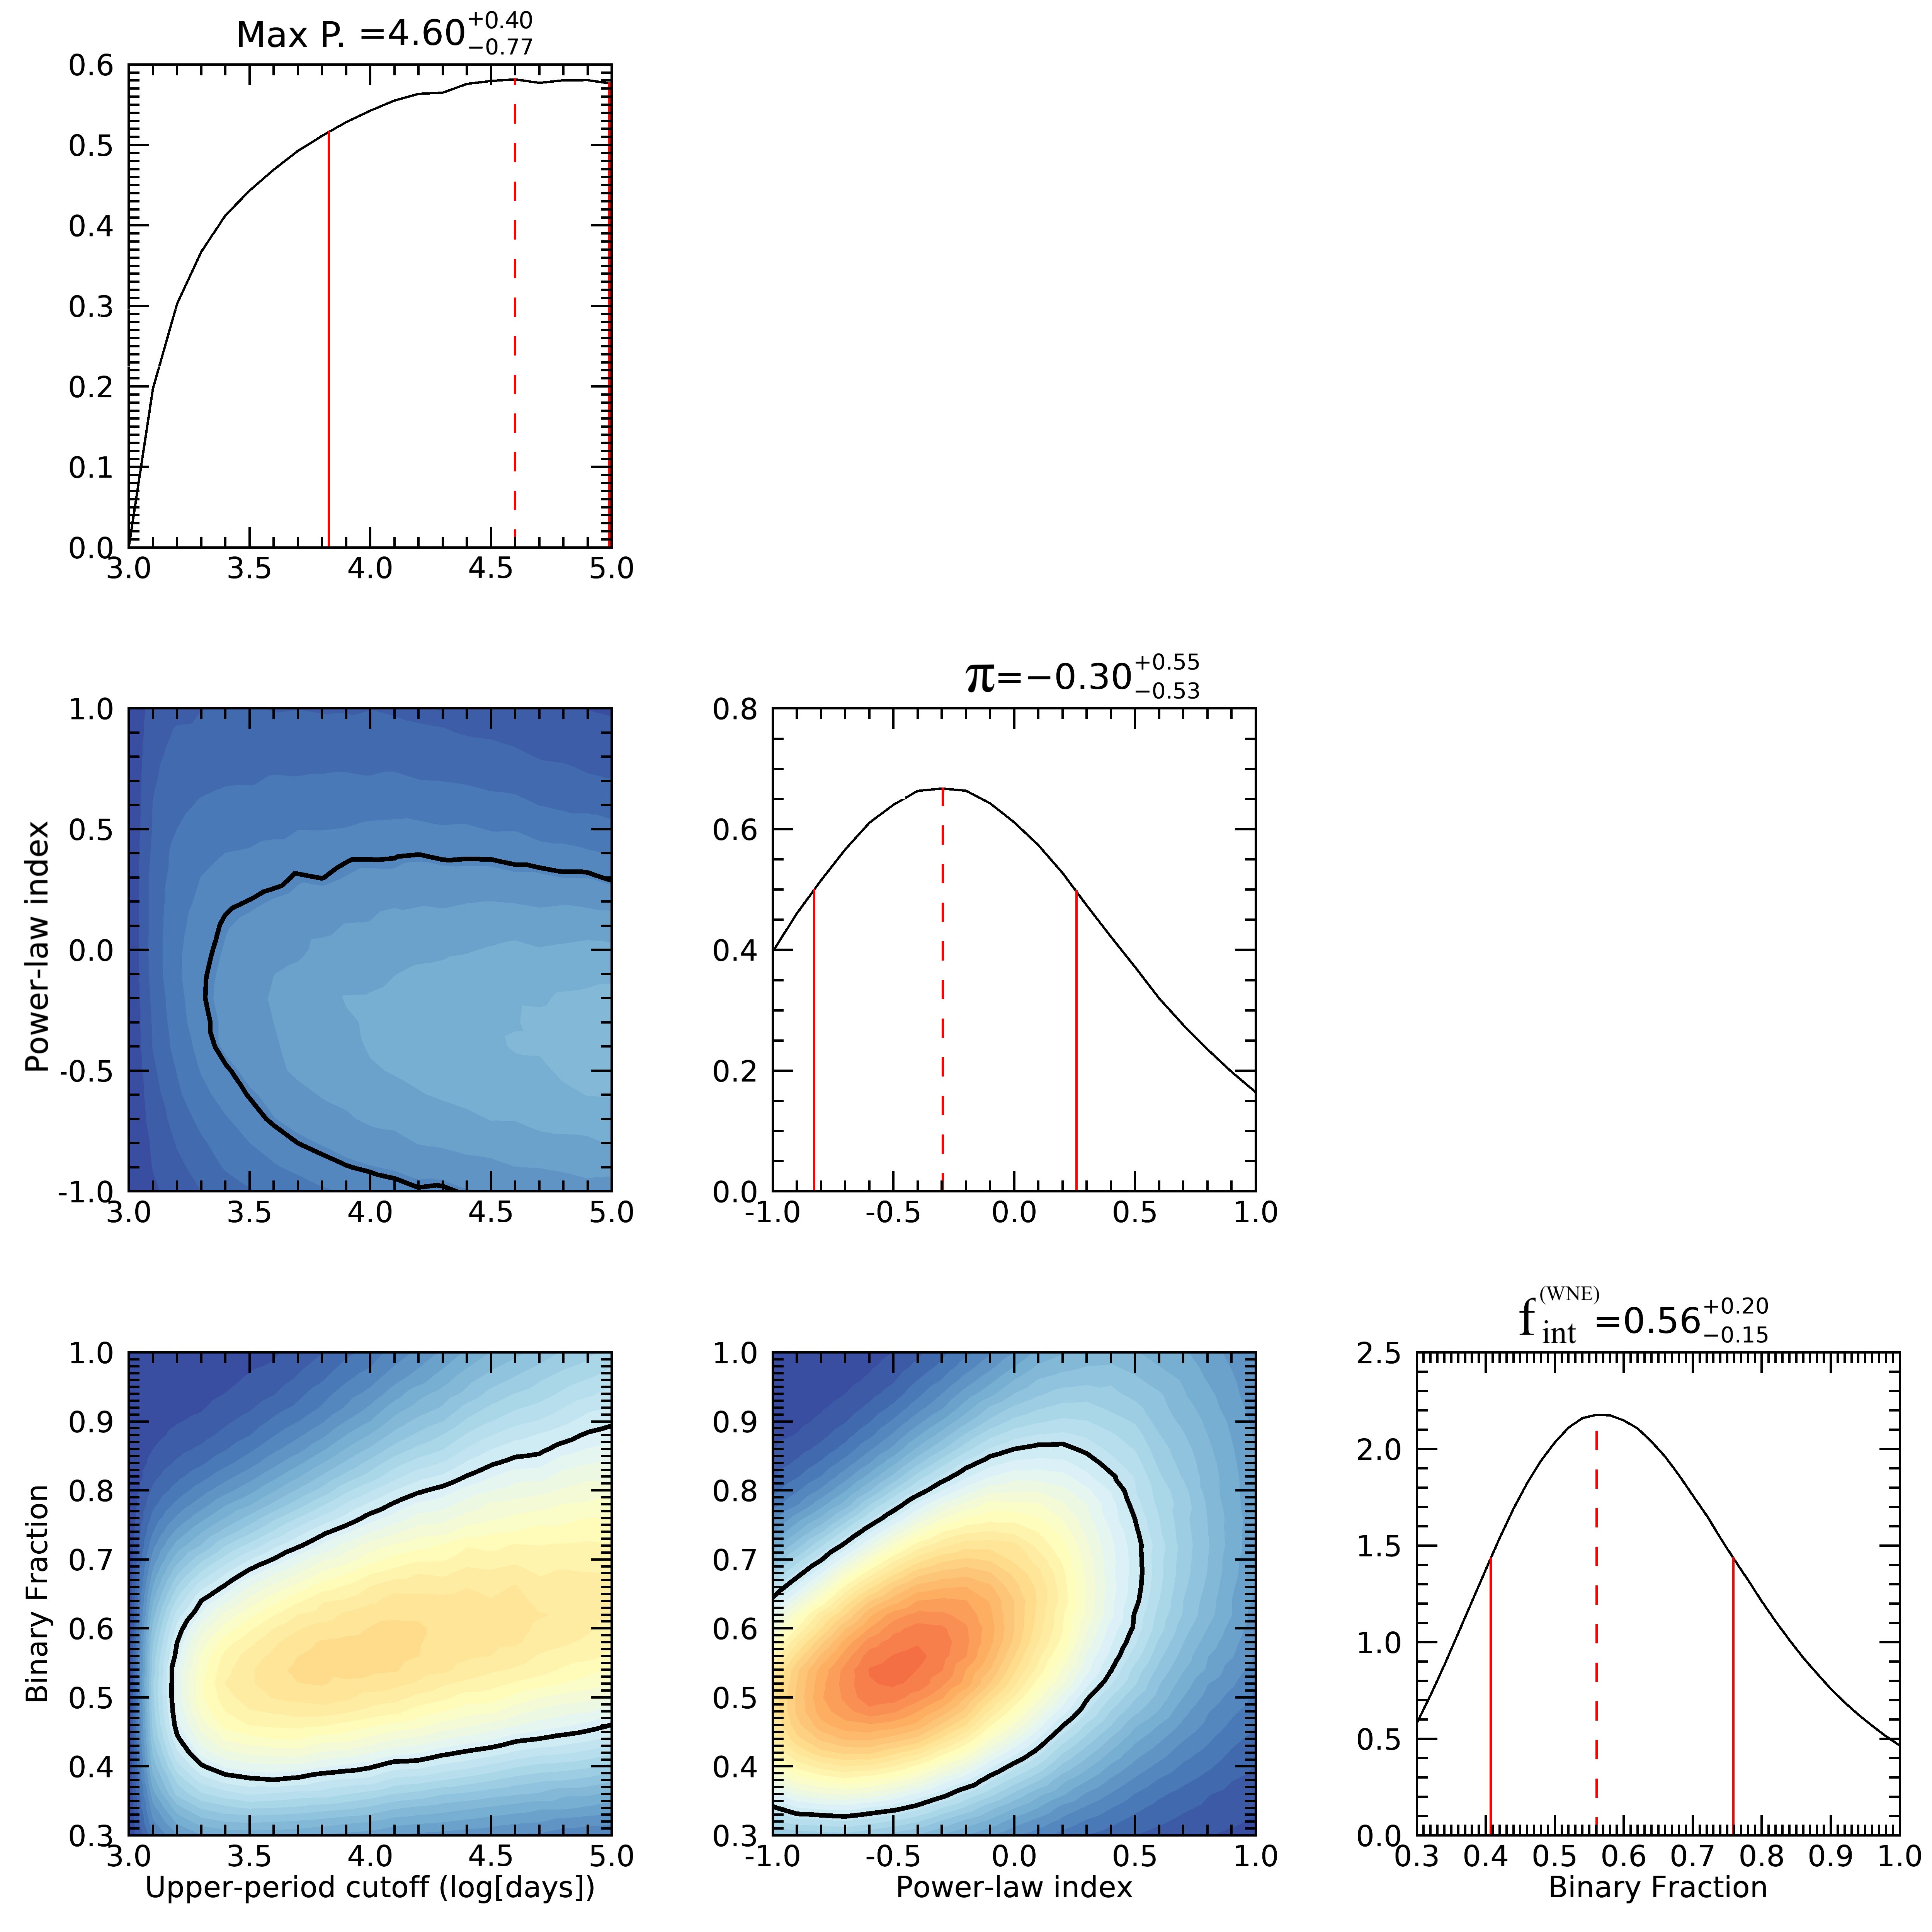
\includegraphics[width=\textwidth]{chapters/WNE/image/WN_AUG30_FPmaxPL_Qmax2_HighRes2_Posterior.png}
    \caption{Three-dimensional likelihood over \logPmax{}, \fintWNE{} , and $\pi$. Assuming flat priors, the one-dimensional posteriors are also shown. For each posterior, the solid red lines show HDI68, and the dashed red line shows the mode.}
    \label{fig:flat_pdist_binfrac}
\end{figure*}

One of the caveats of our simulations is the assumption on the mass ratio distribution. We have assumed a flat distribution between 0.1 and 2. However, this need not be the case in nature, as the outcome of binary interaction scenarios is an important variable. Table \ref{tab:WN_data} shows that known companions around WNE stars are main-sequence O stars (i.e. more massive companions). However, this result may suffer from a bias because binaries with low-mass companions will be much harder to detect. This is because the WR companion will not show much RV variation, and the brightness ratio will make it hard to detect any spectral features of the companion. We therefore decided to explore various power-law indices for the mass ratio distribution ($\kappa$). With the same setup as above, we assumed $\kappa =$ +1.0 and -1.0 for the mass-ratio distribution and computed the same three-dimensional likelihood (Figs. \ref{fig:kappa_plus1} and \ref{fig:kappa_minus1}, respectively). The conclusions from Fig. \ref{fig:flat_pdist_binfrac} did not change significantly, with $\kappa = -1.0$ yielding more short-period binaries\,($\pi = -0.6$) alongside a larger \fintWNE{} of 0.66, and $\kappa = +1.0$ yielding more massive companions with a slightly lower \fintWNE{} of 0.54. In all cases, the constraint on the minimum extent of the period distribution remained similar with \logPmax{}\,$> 3.8$.

\subsection{Revisiting the WC sample}
\label{sect:WC_bayesian}
We reanalysed our results from Chapter \ref{ch:wc} using the improved statistical framework presented in Sect.~\ref{sect:bayesian}. We calculated the four-dimensional likelihood and posteriors for \logPmin{}, \logPmax{}, \fintWNE{} and $\pi$ in order to provide a fair comparison. Unlike in the WNE sample, we did not fix \Pmin{} because we do not have many observational constraints. We explored \logPmin{} from 0.15 up to values of 2.95 and \logPmax{} from 3.0 to 5.0, both in steps of 0.1. In order to fit the absence of short $P$ systems, a low number of intermediate $P$ and a large number of long $P$ binaries, we explored values of $\pi$ from $-1.0$ to $+4.0$ in steps of 0.1. We also explored values of \fintWC{} from 0.30 to 1.00 in steps of 0.02. As in Sects. \ref{sect:detection_probability} and \ref{sect:bayesian}, we assumed a flat distribution for the eccentricity between 0.0 and 0.9, random orientations of the orbital plane in three-dimensional space, and random times of periastron passage.

The WC sample was separated into four \DelRV{} bins: 10\,$\le$\,\DelRV{}\,$\le$\,30\,\kms{} (six objects), 30\,$\le$\,\DelRV{}\,$\le$\,250\,\kms{} (no objects), 250\,$<$\,\DelRV{}\,$\le$\,300\,\kms{} (one object) and  \DelRV{}\,$\ge$\,300\,\kms{} (no objects). We then determined the likelihood of observing the same binned distribution for given values of the four model parameters. We also enforced that our simulations have binaries in the following period bins: $P > 20$\,d (three systems), $P > 2000$\,d (two systems). Assuming a primary mass of 10\,\Msun{}, we simulated 10\,000 populations of 12 WC stars for each bin in this four-dimensional parameter space, hence $\sim 1.1\times10^{10}$ populations. Fig.~\ref{fig:WC_posteriors} shows the four-dimensional likelihood plots along with the one-dimensional posteriors assuming flat priors. The white areas of the plot have a computed likelihood of zero, meaning that none of the 10\,000 populations computed for this set of parameters matched the observations. The HDI68 values are \fintWC{}\,$= 0.96\substack{+0.04 \\ -0.22}$, \logPmin{}\,$= 0.75\substack{+0.26 \\ -0.60}$, \logPmax{}\,$= 4.00\substack{+0.42 \\ -0.34}$ , and $\pi$\,$= 1.90\substack{+1.26 \\ -1.25}$. The values of \fintWC{} and $\pi$ are in agreement with the results of Chapter \ref{ch:wc}, where we found the majority of WC binaries with $P>100$\,d and \fintWC{}\,$> 0.72$.

\begin{figure*}[t]
    \centering
    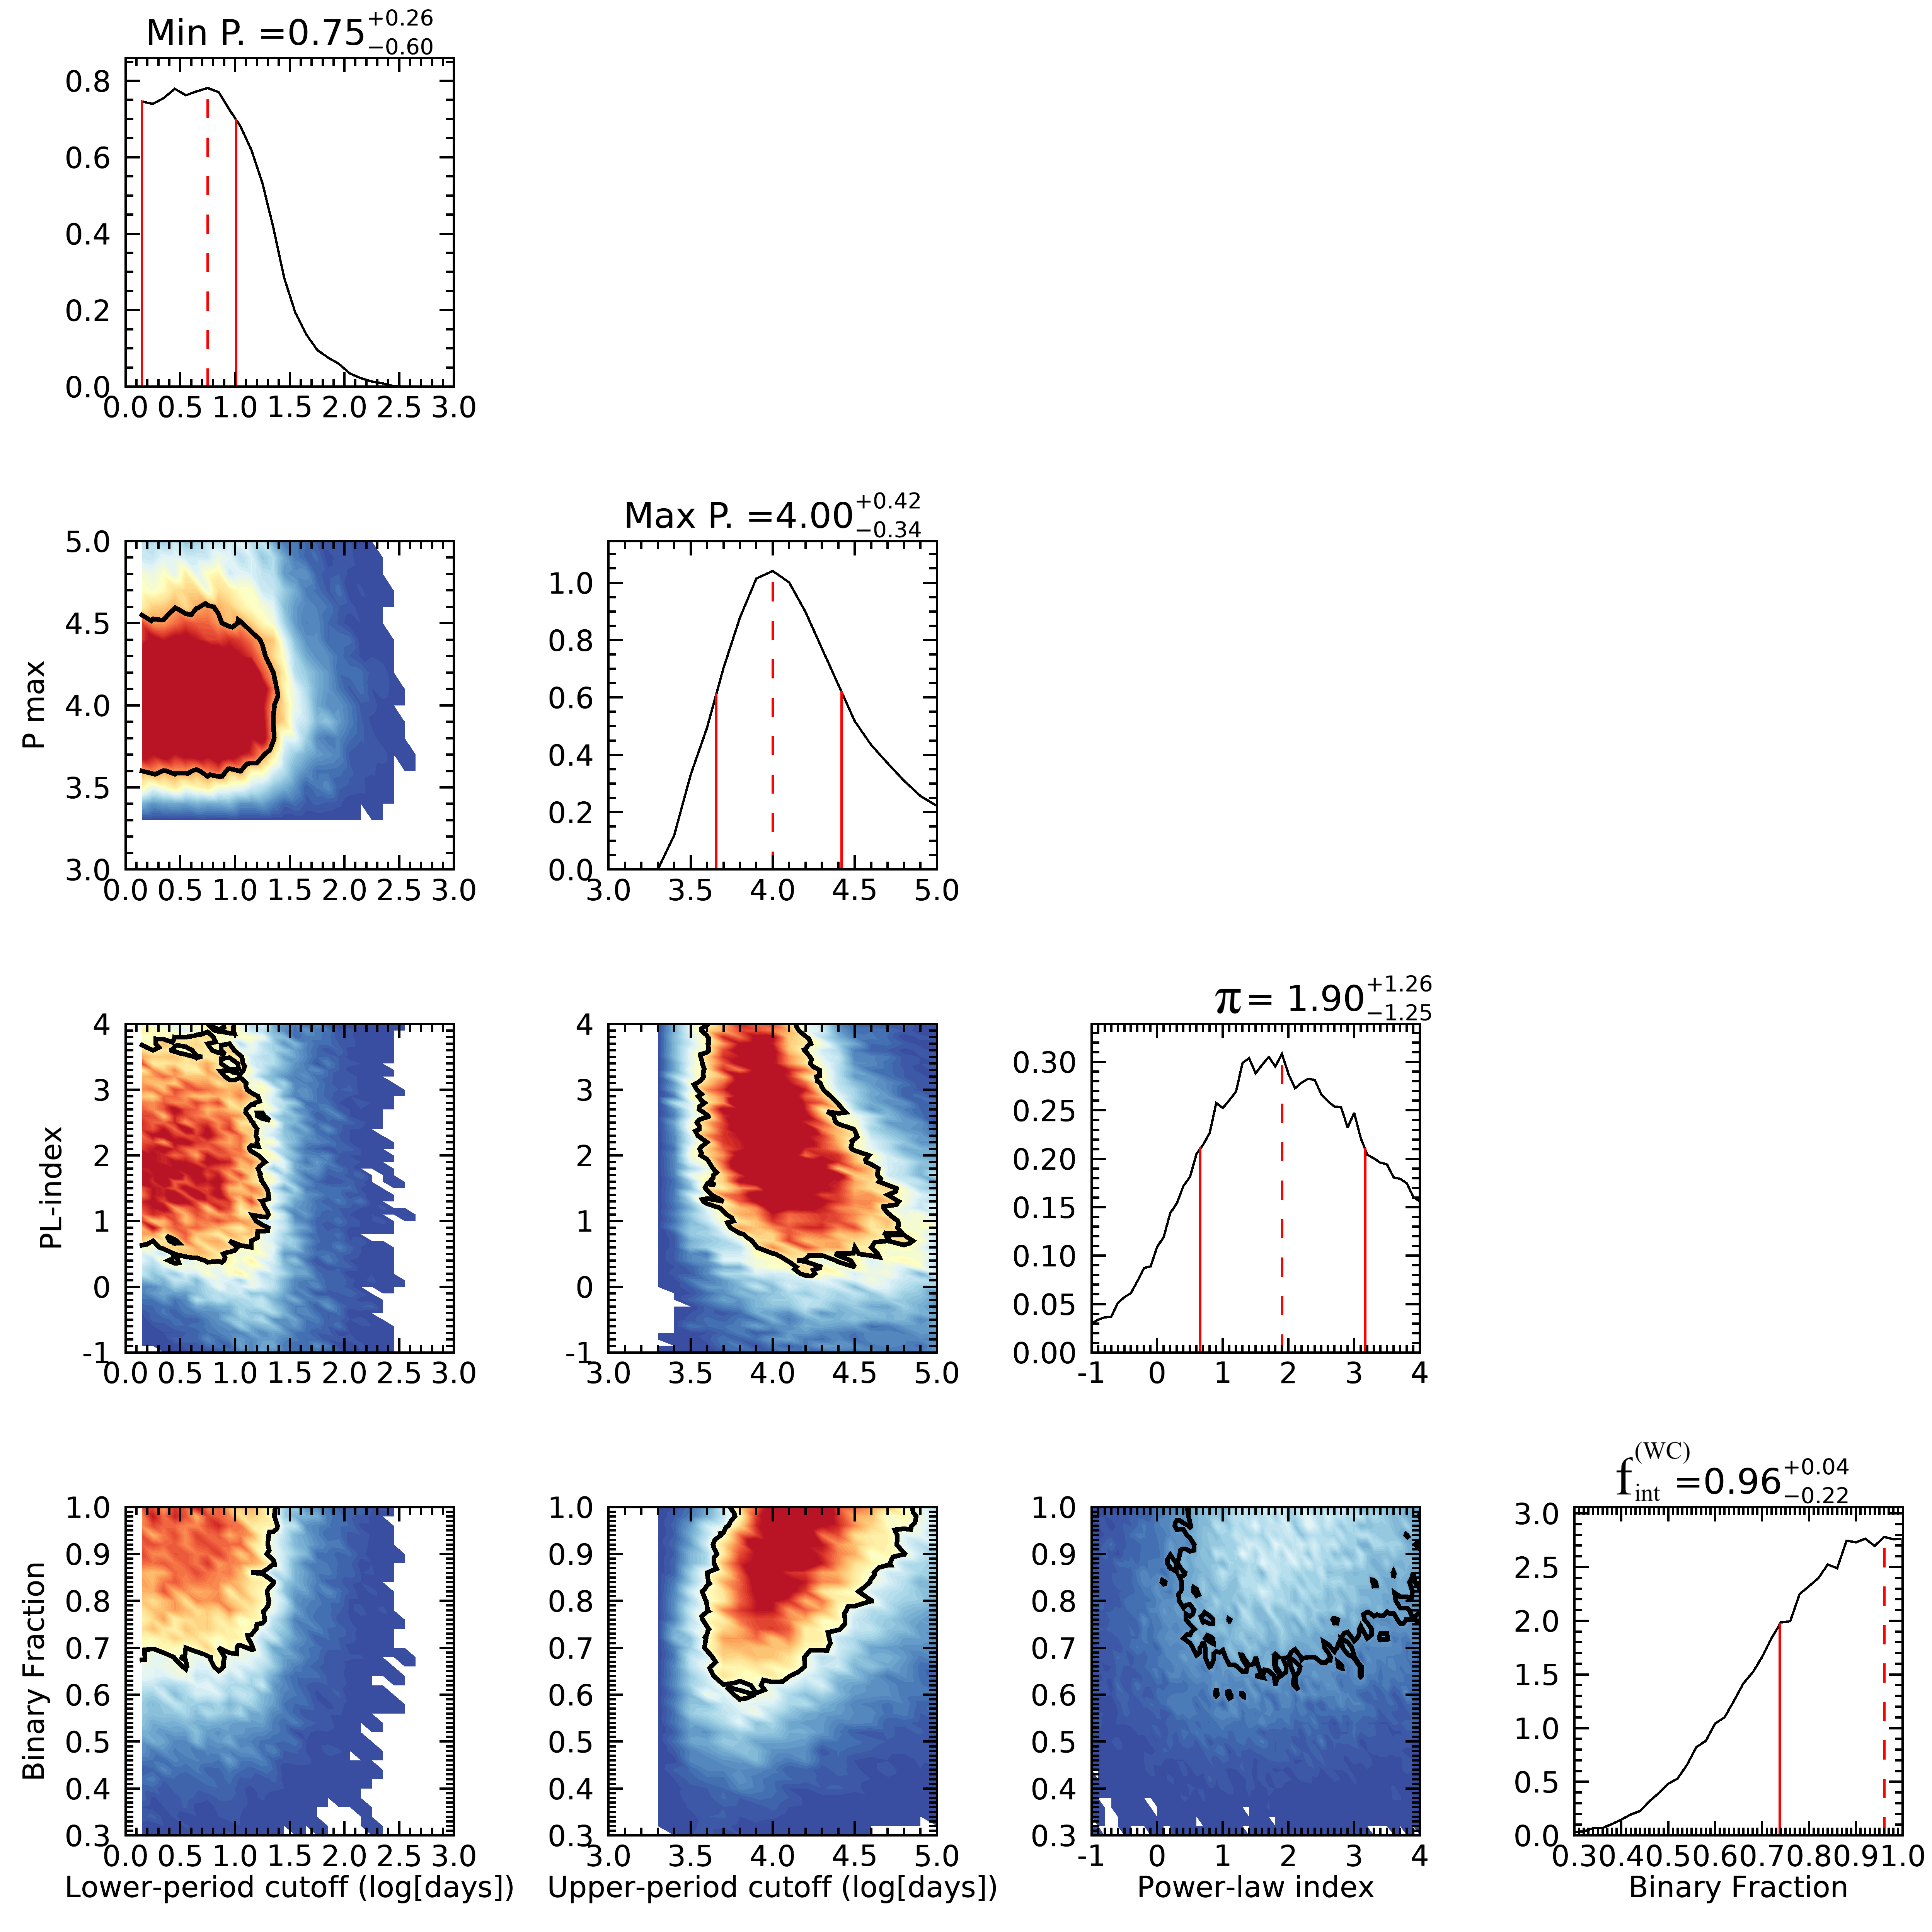
\includegraphics[width=\hsize]{chapters/WNE/image/WC_posterior.png}
    \caption{Four-dimensional likelihood over \logPmin{}, \logPmax{}, \fintWNE{} , and $\pi$ for the WC sample. Assuming flat priors, the one-dimensional posteriors are also shown. For each posterior, the solid red lines show the HDI68, and the dashed red line shows the mode.}
    \label{fig:WC_posteriors}
\end{figure*}

Based on the above analyses, the visualisation of the intrinsic period distributions of the WC and WNE populations is presented in Fig. \ref{fig:periodDistShift}. The period distribution for the WNE population using the best-fit values of \logPmax{} and $\pi$, with \Pmin{} fixed at 1\,d, is shown in red. The solid blue line shows the period distribution for the WC population using the best-fit values of \logPmin{}, \logPmax{} , and $\pi$. In an attempt to express the uncertainties of these parameters on the period distribution, we sampled their posteriors 10\,000 times and over-plot the resulting constructed period distributions. The dark and light shaded areas show 68\% and 95\% of the highest density covered by the distributions, respectively. For the sake of comparison, the distribution for main-sequence O stars from \citet{2012Sana} is also shown (dashed black line).

The derived multiplicity properties might be affected by spectral variability in WR stars on the RV measurements and by the relatively small sample of stars we used. While wind variability in WR stars has a significant effect on the measured RVs, we thoroughly quantified this using our high-cadence studies (Sect. \ref{sect:windVariability} and Chapter \ref{ch:wc}) and statistically accounted for it, using a variability threshold that is high enough to avoid false positives. Similarly, the Bayesian framework presented here accounts for the small sample size. Unless our sample is significantly biased and does not (in a statistical sense) reflect the properties of the parent WNE and WC populations, our conclusions that the WNE and WC stars have different period distributions should hold. We further elaborate on these two aspects in Sects. \ref{sect:literature} and \ref{sect:obsbias_brightness}.

%-------------------------------------- Two column
%
%-----------------------------------------------------------------
\section{Discussion}\label{sect:evolution}

\subsection{Comparison of the binary properties with the literature} \label{sect:literature}

In order to assess whether our results might be biased by the small sample, we explored the literature for statistics on the WNE binary fraction. The GCWR has a total of 387 WN stars, of which 97 are classified as WNE\footnote{As indicated previously, we do not consider WN6 stars to be WNE stars.}. Most of the WR stars in the past decades have been detected through infrared surveys as they are embedded in dust and/or suffer from substantial reddening or extinction, and their multiplicity properties are poorly studied. In order to discuss \fobsWNE{} in the context of a comparable sample that has been well studied for multiplicity, we considered the stars in \citetalias{van_der_hucht_viith_2001}. The catalogue reports a total of 127 WN stars, of which 49 are of the WNE subtype. Of this subset of 49 stars, 13 are WNE binaries with derived spectroscopic orbital solutions. The observed spectroscopic multiplicity fraction for WNE stars in \citetalias{van_der_hucht_viith_2001} is then 0.27.

Table \ref{tab:WN_data} shows that most of
the WNE binary systems in our sample with known periods have periods of a few days to a hundred days. WR 138 is the only long-period binary system with a period of about four years. In \citetalias{van_der_hucht_viith_2001}, all of the other WNE binaries with derived spectroscopic orbital solutions have orbital periods shorter than 15\,d (Fig. \ref{fig:obs_pdist}). Therefore, the observed period distribution of the WNEs in our sample seems to be confirmed with the threefold larger literature-based sample. In contrast to the WC stars studied in Chapter \ref{ch:wc} and a similar literature search \citetalias{van_der_hucht_viith_2001}, there seems to be a systematic skew in the observed period distribution, with a higher frequency of short-period WNE binaries than long-period ones, even in logarithmic space. There is thus no indication that our sample is biased, nor that the results of Sect. \ref{sect:intbinfrac} are contradicted by known WR properties from the existing literature at large.

\subsection{Observational biases due to the magnitude limit} \label{sect:obsbias_brightness}

Considering a population of Galactic WR stars within a certain volume, it is reasonable to assume that the WR stars in binaries will be brighter than the single WR stars \citep{1980VanbeverenConti}. This implies a potential bias due to our selection criterion, which will be larger or smaller depending on the contrast in brightness between the binaries and the single stars.
Because most known WR binaries comprise OB-type companions, we made the simplifying assumption that WR binaries are twice as bright as single WR stars on average \citep[e.g.][]{2019Shenar}. This implies that to avoid this bias, we should include single WR stars in the $V$-band magnitude range 12.0 to 12.7 mag.

In order to investigate this, we explored the GCWR for WNE stars within this magnitude range. For stars with missing $V$-band magnitudes, we searched for $\varv$-band magnitudes between 13.0 and 13.7, similar to our approach in Sect. \ref{sect:sample_WNE}. For the WNE sample, we found two entries, both presumably single stars, WR 126 (WC5/WN) and WR 129 (WN4o). When we conservatively adopt these two targets as single WNE stars, \fintWNE{} changes from 0.56 (9 out of 16) to 0.50 (9 out of 18). This difference is smaller by a factor of three than our errors and is hence negligible.

For the WC sample, we found four new entries in the GCWR. Of these, WR 114 \citep[WC5\,+\,OB?:][]{2001vanderHucht} and WR 132 \citep[WC6\,+\,?:][]{1983BisiacchiWR132} are candidate binaries, WR 125 \citep[WC7ed\,+\,O9III:][]{2019WilliamsNEOWISE,2021AroraWR125} is a confirmed binary, and WR 150 (WC5) is a presumably single star. As was the case with the WNEs, accounting for these objects results in \fintWC{} that is well within the derived uncertainties.

Therefore, the effect of this bias is not significant given our derived values. This can be understood through multiple reasons. \b{First, there is a void of massive star-forming regions at distances between about 3 and 8\,kpc.} While we may be able to detect WRs in the Carina star-forming region (${\sim}$2.7\,kpc), we are unable to detect them in Westerlund 1 (${\sim}$3.8\,kpc) because they suffer from large interstellar extinction \citep{2005Clark}. Second, a notable fraction of WC binaries are dust-producing systems \citep{1995Williamsdust} and hence could experience increased circumstellar reddening. This would cause them to be fainter in the $V$ band, which could balance out the increase in brightness due to additional companions.

\subsection{Implications for binary evolution}

According to our current understanding of stellar evolution \citep{1976Conti,2003MeynetMaeder,2007Crowther}, depending on their initial mass, main-sequence O stars evolve into either cool supergiants or luminous blue variables (LBVs) before becoming WR stars by losing their envelope. Because the spectra of WR stars are thought to reflect the products of fusion in the stellar interiors, the Conti scenario \citep{1976Conti,2007Crowther} proposes a spectroscopic evolution from O stars to the WNL, WNE, WC, and, if they are massive enough, WO phases before these stars end their lives as compact objects. The focus of this section is to use our new multiplicity constraints on the WC (Chapter \ref{ch:wc}) and WNE stars to investigate the evolutionary connections between these various categories of objects.


\begin{figure}
    \centering
    % \includegraphics[width=0.9\textwidth]{Figures/PeriodDistShift.png}
    \includegraphics[width=\textwidth]{chapters/WNE/image/PeriodDistShift.png}
    \caption{Period distributions for main-sequence O stars (dashed black line, from \citet{sana_binary_2012}), WNE stars (red), and WC stars (blue). The WNE and WC distributions are calculated from the posteriors of the MC simulations (Sect. \ref{sect:bayesian}). The posteriors for the WC sample are shown in Fig. \ref{fig:WC_posteriors}.}
    \label{fig:periodDistShift}
\end{figure}

% \subsubsection{Progenitors of WNE binaries}
Following the Conti scenario, WNE stars are thought to have evolved from main-sequence O stars via the WNL phase by wind stripping. As discussed before, the multiplicity parameters of the populations of WNE and O stars are congruous within errors (Sect. \ref{sect:bayesian} and Fig. \ref{fig:periodDistShift}). If the population of binary WNE stars is the product of mass stripping in OB star binaries, similarities between their distributions are to be expected. For example, if a 40\,\Msun{} star becomes a 20\,\Msun{} WNE after transferring its envelope to a companion, the ratio of the pre- and post-interaction period ($P_\mathrm{f}/P_\mathrm{i}$) can be determined analytically given assumptions on mass-transfer efficiency and its companion \citep{1997SobermanMassTransfer}. For the case of a 20\,\Msun{} accretor and conservative mass transfer, $P_\mathrm{f}/P_\mathrm{i}=1$, while for fully non-conservative mass transfer (assuming material is ejected with the specific angular momentum of the accretor), we have $P_\mathrm{f}/P_\mathrm{i}\simeq 0.9$. As an example of a system with an initial mass ratio closer to unity, if the accretor has 35\,\Msun{} at the onset of mass transfer, then $P_\mathrm{f}/P_\mathrm{i}\simeq 2.1$ for conservative mass transfer, while $P_\mathrm{f}/P_\mathrm{i}\simeq 2.7$ for the non-conservative case. Therefore, mass transfer will not significantly modify the period distribution of O stars as they evolve into WNEs, which is compatible with the results of Fig. \ref{fig:periodDistShift}.

If WC stars are direct descendants of WNE stars, the orbital evolution from the WNE to the WC phase is expected to be mainly governed by mass loss due to their stellar winds. This results in the widening of the orbit, so that a shift to longer orbital periods is expected. To quantify this shift, we considered a 20\,\Msun{} WNE star in a binary system with a 30\,\Msun{} main-sequence O star. Even if the WNE star loses 15\,\Msun{} by the time it becomes a WC star, the orbital period of the system would only change by a factor of two. Therefore, only for WNE binaries in the long-period tail ($P>500$\,d) of the inferred distribution can mass loss lead to orbital periods compatible with the peak of the WC distribution ($P>1000$\,d). If indeed WC stars originate from WNE stars losing mass, then explaining the distributions shown in Fig. \ref{fig:periodDistShift} requires that preferentially longer-period WNE binaries evolve into WC stars, while the shorter-period ones avoid that outcome.

A possibility for the longer-period regime is that we simply do not detect WNE binaries with periods greater than a few thousand days in this current RV campaign. This is shown in Fig. \ref{fig:Pdetect_overall}, where our detection probability drops to 40\% at $P\sim1000$\,d and 0\% at $P>10000$\,d. The presence of an undetected long-period population of WNE binaries would indeed provide natural progenitors to the long-period WC binary population. The value of \fintWNE{} would then be much higher than reported here, however. Almost all of the apparently single WNE stars would be in long-period binaries, resulting in a \fintWNE{} close to 1.00.

\section{Conclusions}\label{sect:conclusions_WNE}
We have established the observed and intrinsic multiplicity properties of a complete magnitude-limited sample of 16 northern Galactic WNE stars using data from the HERMES spectrograph since 2017. We measured the RVs using cross-correlation with a statistical framework that allowed us to derive meaningful uncertainties. Adopting a peak-to-peak variability threshold $C$ of 50\,\kms{}, which is more than three times the observed short-term variability for WR 138, we derived an observed spectroscopic binary fraction, \fobsWNE{}, of 0.44\,$\pm$\,0.12.

Using MC simulations, we determined constraints on a parametrised model of the distribution of orbital parameters. In particular, we considered a distribution described by a power-law index $\pi$ and upper and minimum values \logPmin{} and \logPmax{} for the period distribution, as well as the intrinsic binary fraction \fintWNE{}. Assuming flat priors for these model parameters, we found \fintWNE{} to be $0.56\substack{+0.20 \\ -0.15}$. The power-law index for the period distribution, $\pi$, was found to be $-0.30\substack{+0.55 \\ -0.53}$. Both these values are consistent with what was derived for main-sequence O stars by \citet{2012Sana}. Furthermore, the period distribution also favours the majority of systems at orbital periods shorter than 100\,d. This is in stark contrast to what we found for the Galactic WC population (\fintWC{}\,$= 0.96\substack{+0.04 \\ -0.22}$, $\pi$\,$= 1.90\substack{+1.26 \\ -1.25}$.), where the majority of binaries had orbital periods of a few 1000 days. The 68\% highest-density interval values of $\pi$ for the WC and WNE populations do not overlap.

% Taking the discrepancy in the period distributions of the WNE and WC populations at face value in our analyses and in the literature \citepalias[][]{van_der_hucht_viith_2001} questions the presence of a systematic evolutionary connection between WNE and WC stars. A population of WNE binaries at $P\,{\sim}\,1000$\,d appears to be missing. These would be ideal progenitors of the observed WC binaries given the orbital evolution due to mass loss. Secondly, the evolved counterparts of the observed short-period WNE binaries seem to be missing, despite the high sensitivity of the RV campaign in Chapter \ref{ch:wc}. These results, combined with a similar deficit from literature studies, indicate the absence of a corresponding population of short-period WC binaries.

% Considering the populations of main-sequence O stars, WNE and WC stars are linked from an evolutionary standpoint, it is possible for main-sequence O binaries to evolve into WNE binaries through Case A or early Case B mass transfer. However, depending on the initial period, the system would not survive if the initial mass ratio diverged drastically from unity. It is also possible for short-period WNE binaries to form via a common-envelope scenario, which could occur due to either late Case B or Case C mass transfer in a wide main-sequence O binary, regardless of the initial mass ratio. The long-period tail of the WNE period distribution is consistent with the current multiplicity statistics for LBVs \citep{2022Mahy}, possibly indicating an evolutionary sequence from long-period main-sequence O binaries $\rightarrow$ LBV $\rightarrow$ WNE $\rightarrow$ WC.

% The orbital evolution of WNE binaries is mainly governed by mass loss, leading to an expansion of the orbital period by a factor of ${\sim}1.5$-2. This change is insufficient to explain the observed differences between the WNE and WC period distributions, which peak at $P<10$\,d and $P{\sim}5000$\,d, respectively. It thus appears that short-period WN binaries have a low chance of becoming WC binaries, for reasons that are not yet understood.


Considering the fact that WNE stars do go on to strip their envelopes and form WC stars \citep{2003MeynetMaeder}, understanding the orbital evolution of the WNE population as the stars evolve to the WC phase is critical. The change in the orbital period from the WNE to the WC phase is governed by mass-loss through stellar winds, which is of a factor ${\sim}1$-2. While the long-period WNE binaries could evolve via the LBV phase to form WCs, the descendants of short-period WNE binaries is still a mystery.

The existing multiplicity properties gathered from the literature on a larger sample and the smaller but statistically better-characterised sample presented here seem to indicate that the underlying period distributions for WC and WNE populations are different. This can offer substantial diagnostics on the evolution of these systems. However, owing to the significant evolutionary implications from the above discrepancy, it is critical to increase the sample size of such magnitude-limited studies.

\clearpage
\thispagestyle{empty}
\hspace{0pt}
\vfill
\textit{The cemetry is a hot hangout spot with kids these days. Everone is just dying to get in!}
\vfill
\clearpage
